\begin{figure}[H]
\centering
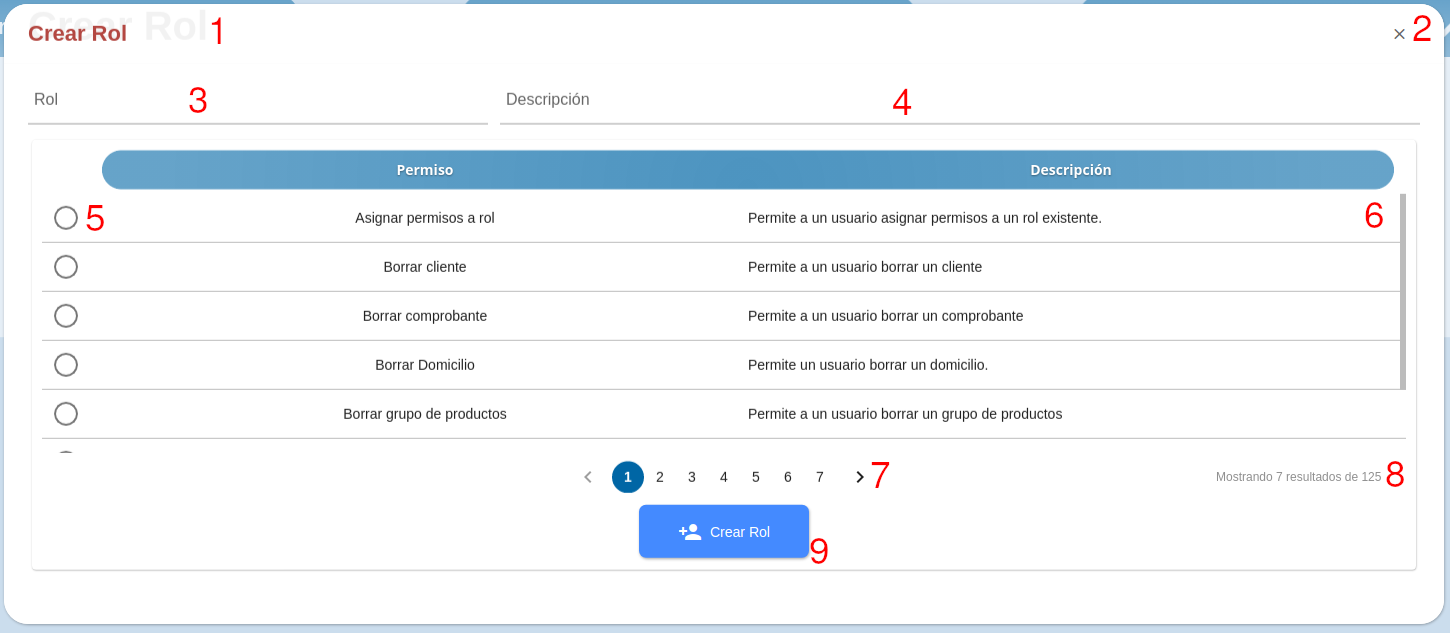
\includegraphics[width=\textwidth,height=\textheight,keepaspectratio]{Escenarios/AD-36-00}
\caption{Escenario - AD-36-00}
\label{fig:AD-36-00}
\end{figure}

Este escenario permite crear o modificar un rol, en \textbf{AD-36-01} se indicará la operación que se esté realizando mostrando 'Crear Rol' o 'Modificar Rol'. Con el botón \textbf{AD-36-02} se podrá volver al escenario \textbf{AD-35-00}. Se debe ingresar un nombre de rol en \textbf{AD-36-03} y si se desea una descripción en \textbf{AD-36-04}. Luego se muestra una tabla con todos los permisos existentes, pudiendo seleccionar con el botón \textbf{AD-36-05} cuáles de ellos desea que tenga el rol que se está creando modificando. En caso de estar modificando, los permisos existentes en el rol estarán pre-seleccionados. En \textbf{AD-36-05} se puede ver información de cada uno de los permisos, mostrando el nombre del permiso y descrpción. En \textbf{AD-36-07} se mostrarán las distintas páginas con todos los permisos, pudiendo navegar entre ellas. En \textbf{AD-36-08} se mostrará cuántos permisos se están visualizando y el total.
Al hacer click en el botón \textbf{AD-36-09} se modificará o creará el rol según corresponda, mostrando en el botón el texto 'Crear Rol' o 'Modificar Rol' respectivamente, asignando los permisos que hayan sido seleccionados al rol.
\clearpage
